% \newpage
\section{Experiments}
\label{sec:experiments}

We conduct extensive experiments to answer the following questions:
% Our experiments mainly focus on the following questions:

\textbf{Q1)} Is a single modality enough to perform efficiently on challenging environments?

\textbf{Q2)} How does our method compare with state-of-the-art imitation learning policies?

\textbf{Q3)} What kinds of fusion types are most powerful?
% \todo[inline]{Please answer these questions somewhere if you state them here, i.e., reference Q1)-Q3)}
%%%%%%%%%%%%%%%%%%%%%%%%%%%%%%%%%%%%%%%%%%%%%%%%%%%%%%%%%%%%%%%%%%%%%%%%%%%%%%
\begin{comment}
\begin{table*}[t]
\centering
\begin{tabular}{llcccccc}
\toprule
\textbf{Methods}& \textbf{Model}& \textbf{Type}  & \textbf{Easy} & \textbf{Medium} & \textbf{Hard} & \textbf{Extra} & \textbf{All} \\  
\midrule 
SYN-SQL & Sense 13B & SFT & 95.2\% & 88.6\% & 75.9\% & 60.3\% & 83.5\% \\  
SQL-Palm & PaLM2 & SFT& 93.5\% & 84.8\% & 62.6\% & 48.2\% & 77.3\% \\ 
CPO-SQL &  & SFT& \% & \% & \% & \% & \% \\ 
\hline
DIN-SQL & GPT-4 & Zero-shot & 91.1\% & 79.8\% & 64.9\% & 43.4\% & 74.2\% \\  
C3q-SQL & GPT-4 & Zero-shot & 82.0\% &57.0 \% & 54.6\% & 47.1\% & 61.0\% \\  \hline
    DAIL-SQL  &  GPT-4 & Few-shot& 90.7\% & \textbf{89.7\%} & 75.3\% & 62.0\% & 83.1\% \\ 
ACT-SQL  &  GPT-4 & Few-shot& 91.1\% & 79.4\% & 67.2\% & 44.0\% & 74.5\% \\
PTD-SQL  & GPT-4 & Few-shot& 94.8\% & 88.8\% & 85.1\% & 64.5\% & 85.7\% \\ 
PTD-SQL  & GPT-4 & Few-shot& 94.8\% & 88.8\% & 85.1\% & 64.5\% & 85.7\% \\ 
\hline
\textit{\textbf{ \textit{SAL-SQL}}}& GPT-4& Zero-shot & \textbf{93.8\%} & {87.9}\% & 88.5\% & 74.2\% & 87.1\% 
\\  
\textit{\textbf{ \textit{SAL-SQL}}}& Llama3.1-8B-Instruct& Zero-shot & {73.2\%} & {76.1}\% & {63.2\%} & {59.4\%} & {70.5\%} 

\\
\textit{\textbf{ \textit{SAL-SQL}}}& Deepseek-coder-6.7B & Zero-shot & {88.8\%} & {65.5}\% & {63.8\%} & {25.3\%} & {64.2\%} 

\\
\textit{\textbf{ \textit{SAL-SQL}}}& Qwen2.5-7B-Instruct & Zero-shot & {83.6\%} & {80.7}\% & {78.7\%} & {69.4\%} & {79.2\%} 

\\ 
\textit{\textbf{ \textit{SAL-SQL}}}& Starcoder2-7B& Zero-shot & {89.2\%} & 88.9\% & {84.5\%} & {70.6\%} & {85.2\%} 
\\
\textit{\textbf{ \textit{SAL-SQL}}}& GPT-4o-mini& Zero-shot & 93.6\% & {87.5}\% & \textbf{90.1\%} & \textbf{74.7\%} & \textbf{87.4\%} 
\\  
\bottomrule
\end{tabular}
\caption{Execution accuracy performance of different methods across difficulty levels of spider dev set.}
\label{tab:sql_comparison}
\end{table*}
\end{comment}

\begin{table}[t]
\setlength{\tabcolsep}{3pt} % Default is usually 6pt
\centering
\resizebox{\columnwidth}{!}{
\small
%\normalsize	
\begin{tabular}{llccccc}
\toprule
\textbf{Method} & \textbf{Model} & \textbf{Easy} & \textbf{Medium} & \textbf{Hard} & \textbf{Extra} & \textbf{All} \\ 
\midrule
\multicolumn{7}{c}{\textbf{Supervised Fine-Tuning (SFT)}} \\
\midrule
SYN-SQL    & Sense 13B           & \textbf{95.2} & 88.6 & 75.9 & 60.3 & 83.5 \\  
SQL-Palm   & PaLM2               & 93.5 & 84.8 & 62.6 & 48.2 & 77.3 \\  
% CPO-SQL    & --                  & --     & --     & --     & --     & --     
\midrule
\multicolumn{7}{c}{\textbf{Zero-shot Methods}} \\
\midrule
Baseline   & GPT-4                & 84.3 & 73.1 & 65.8 & 40.3 & 69.1 \\   
Baseline   & GPT-4o                & 87.2 & 77.2 & 68.4 & 48.7 & 73.4 \\  
Baseline   & GPT-4o-mini          & 84.8 & 75.6 & 67.0 & 46.1 & 71.5  \\    
C3q-SQL    & GPT-4                & 90.2 & 82.8 & 77.3 & 64.3 & 80.6 \\  
\midrule
\multicolumn{7}{c}{\textbf{Few-shot Methods}} \\
\midrule
DIN-SQL    & GPT-4                & 91.1 & 79.8 & 64.9 & 43.4 & 74.2 \\ 
DAIL-SQL   & GPT-4                & 90.7 & \textbf{89.7} & 75.3 & 62.0 & 83.1 \\ 
ACT-SQL    & GPT-4                & 91.1 & 79.4 & 67.2 & 44.0 & 74.5 \\
PTD-SQL    & GPT-4                & \underline{94.8} & 88.8 & 85.1 & 64.5 & 85.7 \\ 
DEA-SQL    & GPT-4                & 88.7 & \underline{89.5} & 85.6 & 70.5 & 85.6 \\ 
\midrule
\multicolumn{7}{c}{\textbf{Self-augmented In-Context Learning}} \\
\midrule
SAFE-SQL    & GPT-4                & 93.2 & 88.9 & \underline{85.8} & 74.7 & 86.8 \\ 
SAFE-SQL    & GPT-4o                & 93.4 & 89.3 & \textbf{88.4} & \textbf{75.8} & \textbf{87.9} \\
SAFE-SQL    & GPT-4o-mini         & 93.6  & 87.5 & 86.1 & \underline{75.2} & \underline{87.4} \\
\bottomrule
\end{tabular}
}
\caption{Execution accuracy across difficulty levels on the Spider development set. The highest score per row is in bold, and the second highest is underlined.}
\vspace{-3mm}
\label{tab:sql_comparison}
\end{table}

%%%%%%%%%%%%%%%%%%%%%%%%%%%%%%%%%%%%%%%%%%%%%%%%%%%%%%%%%%%%%%%%%%%%%%%%%%%%%%

\subsection{Simulations}

\textbf{RoboCasa} \cite{robocasa2024}:
RoboCasa is a large-scale simulation framework designed to train generalist robots in diverse and realistic household environments, with a particular emphasis on complex kitchen tasks. It features 120 meticulously crafted kitchen scenes, over 2,500 high-quality 3D objects across 150 categories, and 100 tasks divided into foundational atomic tasks and intricate composite tasks. Leveraging generative AI tools, RoboCasa achieves unparalleled diversity, realism, and scalability in robotic learning.
This benchmark is characterized by its exceptional difficulty, stemming from the highly diverse scenarios it presents. Each scenario is accompanied by only one demonstration, significantly increasing the challenge for learning algorithms. For instance, in pick-and-place tasks, the object to be manipulated varies across scenarios, with just one demonstration per case. Furthermore, the training and evaluation datasets feature completely distinct scenes, further testing a model’s ability to generalize and adapt robot behaviors to novel scenarios.
With its extensive task set, environmental variability, and high-fidelity simulations, RoboCasa establishes itself as a new standard for evaluating robotic learning methodologies, pushing the boundaries of generalization and adaptability in robot learning.

\textbf{Training and Evaluation}: We train each method for 100 epochs and rollout the models for 50 times for all tasks in RoboCasa. We group similar tasks together as shown in Table \ref{tab:task_groups} and train the models for each of the groups. 

\subsection{Baselines}

\textbf{BC} \cite{robocasa2024}: We inherit the result reported in RoboCasa. RoboCasa uses the BC-Transformer implemented by RoboMimic. The BC policy uses a CLIP model to encode the goal instruction and a ResNet-18 with FilM layers to encode the image-based observations.

\textbf{3D Diffusion Policy (DP3)} \cite{ze20243d}: DP3
extracts point-wise features from single-view points clouds with a MLP-based encoder and forms a compact 3D visual representation. Robot actions are then generated by a convolutional network-based architecture, conditioned on this representation and the current robot states.

\textbf{3D Diffuser Actor (3DA)} \cite{ke20243d}: 3DA is a diffusion-based policy conditioned on 3D scene features and language instructions.
The 3D scene features are extracted and aggregated from single or multi-view images and depth maps. The policy denoises rotation and translation of the robot's end-effector as action.

\subsection{FPV-Net}
\label{sec:proposed_models}

We systematically evaluate how the FPV-Net deals with different modalities while maintaining a consistent architecture and diffusion policy configuration across all experiments. This setup allows us to directly compare the effectiveness of different representations.

\textbf{PC-only}:
We first group the point cloud by selecting 256 centers via Furthest Point Sampling (FPS), then retrieve 32 nearest neighbors using K-Nearest Neighbors (KNN) to form 256 point groups. Each group is passed through a lightweight MLP encoder, obtaining an embedding per group. These embeddings, along with a language embedding from CLIP, a timestep embedding, and the noisy action, are provided to a transformer-based diffusion policy.

\textbf{RGB-only}:
In this model, each camera view is processed by a ResNet-18 model, which is pretrained and then finetuned separately for each view. FiLM layers condition the network on the CLIP-encoded language instruction. The resulting embeddings from all camera views are subsequently given to the same transformer-based diffusion policy employed in the PC-only model.
% \usepackage{multirow}
% \usepackage{booktabs}


\begin{table}[h]
	\centering
	\caption{Model performance under two coefficient fusion methods.}
	\begin{tabular}{c|ccc} 
		\toprule
		\multirow{2}{*}{Fusion mode} & \multicolumn{3}{c}{R40}                           \\
		& Easy           & Moderate       & Hard            \\ 
		\hline
		straight                     & 90.92          & 82.84          & 80.29           \\
		our                          & \textbf{91.96} & \textbf{83.31} & \textbf{80.59}  \\
		\bottomrule
	\end{tabular}
\label{tabel6}
\end{table}

\textbf{PC+RGB}:
This variant simply concatenates the point group embeddings from PC-only with the RGB embeddings from RGB-only, and feeds the combined representation into the transformer-based diffusion policy.

\textbf{FPV-MLP}:
% \todo[inline]{What is the c. standing for?}
Here, the point cloud is processed as before, but we additionally exploit local RGB features. Specifically, we use the 8x8 feature map produced by the third ResNet layer for each image. This feature map is flattened and concatenated with the global ResNet embedding, producing 65 tokens per view. Tokens from all views, along with a learnable class token, are passed to a transformer. The output of the class token serves as the condition vector for AdaLN, while the point group embeddings enter the diffusion policy in the usual way. 

\textbf{FPV-SUGAR}:
In this model, we use the point cloud encoder of the pretrained 3D visual representation model SUGAR \cite{Chen_2024_SUGAR}, which also partitions points into 256 groups of 32 via FPS and KNN, but subsequently also employs a 12-layer transformer. We use the model pretrained on multi-object scenes using objects from the Objaverse \cite{objaverse} dataset. To reduce computational cost, we freeze the first 10 layers and finetune only the last 2. The RGB images are processed similarly to FPV-MLP, except that we use the 4x4 feature map from the fourth ResNet layer. Finally, the conditioned transformer-based diffusion policy is applied as before.

\subsection{Main Results}


Table \ref{table:main_results_2d} shows that models utilizing both modalities outperform those using a single modality, which addresses Q1. Simply concatenating point cloud and RGB features leads to a 10\% improvement, illustrating the complementary nature of spatial and semantic information: each modality contributes unique advantages that are not fully captured by the other. Notably, pick-and-place and insertion tasks benefit most from having both modalities, suggesting that both spatial and semantic cues are crucial for manipulating objects unseen during training.
In one particular task the PC-only method performs noticeably better than the other models, namely the \textsc{TurnSinkSpout} task, which requires further investigation.
\begin{figure}
    \centering
    \resizebox{0.48\textwidth}{!}{% Scale to half the page width
    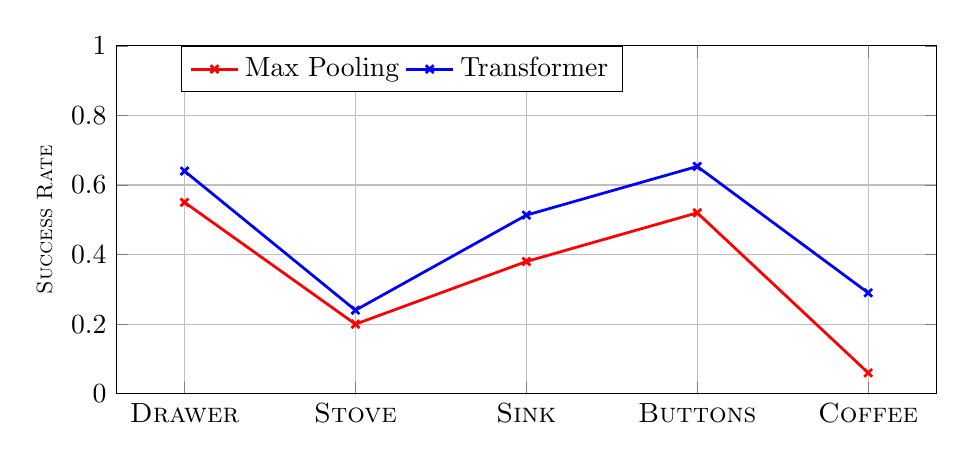
\begin{tikzpicture}[baseline]
    \definecolor{lightgray204}{RGB}{204,204,204}
    \definecolor{crimson}{RGB}{214,39,40}
    \definecolor{darkgray}{RGB}{176,176,176}
    \definecolor{darkorange}{RGB}{255,127,14}
    \definecolor{darkturquoise}{RGB}{23,190,207}
    \definecolor{forestgreen}{RGB}{44,160,44}
    \definecolor{goldenrod}{RGB}{188,189,34}
    \definecolor{gray}{RGB}{127,127,127}
    \definecolor{mediumpurple}{RGB}{148,103,189}
    \definecolor{orchid}{RGB}{227,119,194}
    \definecolor{sienna}{RGB}{140,86,75}
    \definecolor{steelblue}{RGB}{31,119,180}
    
    \begin{axis}[
        height=6cm,
        width=12cm,
        bar width=3.5pt,
        ylabel=Success Rate,
        ylabel style={
            font=\footnotesize\scshape
        },
        ymin=0, ymax=1,
        legend style={at={(0.348, 1)}, anchor=north, legend columns=-1},
        symbolic x coords={drawer, stove, sink, buttons, coffee},
        xtick=data,
        % Override the actual tick labels with capitalized names:
        xticklabels={Drawer,Stove,Sink,Buttons,Coffee},
        xticklabel style={font=\scshape},
        ymajorgrids,
        grid=both,
    ]
    
    % -- Max Pooling (red) --
    \addplot [
        draw=red,
        line width=1pt,
        mark=x,
        mark options={solid},
    ]
    coordinates {
        (drawer, 0.5500)
        (stove, 0.2000)
        (sink, 0.3800)
        (buttons, 0.5200)
        (coffee, 0.0600)
    };
    
    % -- Transformer (blue) --
    \addplot [
        draw=blue,
        line width=1pt,
        mark=x,
        mark options={solid},
    ]
    coordinates {
        (drawer, 0.6400)
        (stove, 0.2400)
        (sink, 0.5133)
        (buttons, 0.6533)
        (coffee, 0.2900)
    };
    
    \legend{Max Pooling, Transformer}
    \end{axis}
    
    \end{tikzpicture}
    }
    \caption{Success rates using max pool or transformer to obtain global feature vector of RGB images to use in AdaLN conditioning.}
    \label{fig:ablation_cond_vec}
\end{figure}


Our PC-only approach outperforms 3D Diffusion Policy by a margin of 5.25\%, answering Q2. A likely explanation is that the max-pooling step discards spatial information critical to the diffusion policy. By contrast, our approach retains more of the point cloud’s geometric structure. Furthermore, grouping points instead of handling each point separately like DP3 allows our PC-only model to better capture local spatial features.

FPV-MLP and FPV-SUGAR, conditioning on RGB features, offer further gains, yielding an average success rate of around 50\%, higher than the simple concatenation of modalities. This suggests the diffusion policy exploits the rich texture and semantic details from RGB data when using AdaLN for conditioning more effectively than taking these features purely as an additional input. Another possible reason is that the transformer-based diffusion policy can better separate the two modalities, focusing on spatial relations through self-attention over point groups while annotating each group with semantic features via AdaLN conditioning.

3DA exhibits a very low success rate on RoboCasa in our experiments. This may be attributed to our decision to train each model for 100 epochs to ensure a fair comparison. However, as a relatively more complex model, 3DA likely requires a longer training duration to achieve optimal performance.


\subsection{Ablation on different fusion}


We compared the performance of different fusion strategies for integrating point cloud and RGB embeddings within the transformer architecture. Concat. refers to a straightforward concatenation of both embeddings. Cond. on PC denotes using RGB features as the main modality while conditioning on point cloud features through AdaLN conditioning. Conversely, Cond. on RGB treats point cloud features as the primary modality, with RGB features providing the conditioning signal via AdaLN. As shown in Figure \ref{fig:ablation_fusion}, conditioning the RGB-based transformer on point cloud features underperforms compared to simple concatenation. This could be due to compressing the entire point cloud into a single vector, which may discard crucial spatial details, particularly for tasks like \textsc{Coffee}, where precise grasping of a mug is required. In contrast, conditioning on RGB features yields the best performance across most tasks, effectively addressing Q3.

% We explored various strategies for combining the point cloud and RGB embeddings within the transformer. One option is to concatenate both embeddings and provide them jointly to the transformer. Another approach is AdaLN conditioning, as described in Section \ref{sec:adaln}. Figure \ref{fig:ablation_fusion} shows that using point cloud features to condition the RGB-based transformer performs worse than straightforwardly concatenating the two feature sets. This might be because compressing the entire point cloud into a single vector discards the spatial details needed for tasks like \textsc{Coffee}, where a mug must be grasped. On the other hand, conditioning on RGB features achieves the best performance in most tasks, addressing Q3.


\newcommand{\D}{8} % number of dimensions (config option)
\newcommand{\U}{10} % number of scale units (config option)

\newdimen\R % maximal diagram radius (config option)
\R=3.5cm 
\newdimen\L % radius to put dimension labels (config option)
\L=4cm
\newdimen\B
\B=4.2cm
\newdimen\C
\C=3.8cm

\newcommand{\A}{360/\D} % calculated angle between dimension axes

\begin{figure}
    \centering
    \includegraphics[width=0.4\textwidth]{figure_and_table/ablation/rgb_features_legend_2.pdf}
    \begin{sc}
    \resizebox{0.4\textwidth}{!}{ % Scale the figure to 50% of the page width
        \begin{tikzpicture}[scale=1]
            \path (0:0cm) coordinate (O); % define coordinate for origin

            % draw the spiderweb
            \foreach \X in {1,...,\D}{
                \draw (\X*\A:0) -- (\X*\A:\R);
            }

            \foreach \Y in {0,...,\U}{
                \foreach \X in {1,...,\D}{
                    \path (\X*\A:\Y*\R/\U) coordinate (D\X-\Y);
                    % \fill (D\X-\Y) circle (1pt);
                }
                \draw [opacity=0.3] (0:\Y*\R/\U) \foreach \X in {1,...,\D}{
                    -- (\X*\A:\Y*\R/\U)
                } -- cycle;
            }

            % define labels for each dimension axis (names config option)
            \path (1*\A:\L) node (L1) {PnP1};
            \path (2*\A:\C) node (L2) {PnP2};
            \path (3*\A:\L) node (L3) {Doors};
            \path (4*\A:\B) node (L4) {Drawer};
            \path (5*\A:\L) node (L5) {Stove};
            \path (6*\A:\C) node (L6) {Sink};
            \path (7*\A:\L) node (L7) {Buttons};
            \path (8*\A:\B) node (L8) {Coffee};

            % global
            \draw [color=red,line width=1.5pt]
                ($(D1-1)!0.5!(D1-2)$) --
                ($(D2-1)!0.7!(D2-2)$) --
                ($(D3-8)!0.45!(D3-9)$) --
                ($(D4-6)!0.4!(D4-7)$) --
                ($(D5-2)!0.4!(D5-3)$) --
                ($(D6-5)!0.133!(D6-6)$) --
                ($(D7-6)!0.533!(D7-7)$) -- cycle;

            % 4x4
            \draw [color=green,line width=1.5pt]
                ($(D1-1)!0.4!(D1-2)$) --
                ($(D2-1)!0.35!(D2-2)$) --
                ($(D3-7)!0.85!(D3-8)$) --
                ($(D4-7)!0.8!(D4-8)$) --
                ($(D5-3)!0.5!(D5-4)$) --
                ($(D6-4)!0.667!(D6-5)$) --
                ($(D7-8)!0.667!(D7-9)$) --
                ($(D8-3)!0.4!(D8-4)$) -- cycle;

            % 8x8
            \draw [color=blue,line width=1.5pt]
                ($(D1-1)!0.3!(D1-2)$) --
                ($(D2-1)!0.5!(D2-2)$) --
                ($(D3-8)!0.25!(D3-9)$) --
                ($(D4-7)!0.6!(D4-8)$) --
                ($(D5-2)!0.9!(D5-3)$) --
                ($(D6-6)!0.8!(D6-7)$) --
                ($(D7-8)!0.2!(D7-9)$) --
                ($(D8-4)!0.2!(D8-5)$) -- cycle;

            \draw[<->, very thick, draw=brown, text=brown]
                ($(D1-7)!0!(D1-8)$)
             -- ($(D1-8)!0!(D1-9)$)
                node[midway, above, yshift=4.5pt, xshift=-1.5pt, inner sep=1pt]
                {\textbf{0.10}};

            
        \end{tikzpicture}
    }
    \end{sc}
    \caption{Success rates of conditioning on ResNet features with different granularity level. Each level in the chart corresponds to a 10\% difference in success rate.}
    \label{fig:ablation_rgb_features}
    \vspace{-0.3cm}
\end{figure}

\subsection{Ablation on obtaining condition vector}


AdaLN does not directly support sequences as input, so a single token must be extracted to condition on point clouds or RGB features. We compare two methods: (1) a simple max-pooling layer, and (2) a transformer whose learnable class token serves as the global representation. Figure \ref{fig:ablation_cond_vec} indicates that the transformer-based approach consistently outperforms max pooling in all tested tasks.


\subsection{Ablation on RGB features}
In order to identify the influence of global tokens and local tokens from ResNet feature map, we evaluate FPV-Net with different feature granularity: global features versus 4x4 or 8x8 feature maps. The results are presented in Figure \ref{fig:ablation_rgb_features}, which show that by adding local features from ResNet would gain performance significantly on most tasks such as \textsc{Buttons} and \textsc{Drawers}, whereas the \textsc{Doors} task show less sensitivity. This contrast could be due to the smaller size of buttons and drawer handles, which require finer-grained feature maps for accurate manipulation.

% As mentioned in Section~\ref{sec:proposed_models}, FPV uses a transformer to obtain a condition vector from ResNet features across multiple views when conditioning on RGB. We evaluate different feature granularity: global features versus 4x4 or 8x8 feature maps. Figure \ref{fig:ablation_rgb_features} reveals that some tasks, such as \textsc{Buttons} and \textsc{Drawers}, benefit from local semantic information, whereas tasks in \textsc{Doors} show less sensitivity. This contrast likely stems from the smaller size of buttons and drawer handles, which require finer-grained feature maps for accurate manipulation.


\subsection{Ablation on finetuning SUGAR}

Finally, we examine the effect of different finetuning strategies on FPV-SUGAR. Figure \ref{fig:ablation_sugar_ft} compares a fully frozen SUGAR encoder with an encoder in which only the last two layers are finetuned. With the exception of the stove task, finetuning the last two layers improves performance in nearly every scenario, providing a 2\% boost in average success rate. Finetuning even more layers could potentially further increase the performance of the model.

\begin{figure}
    \centering
    \resizebox{0.48\textwidth}{!}{%
        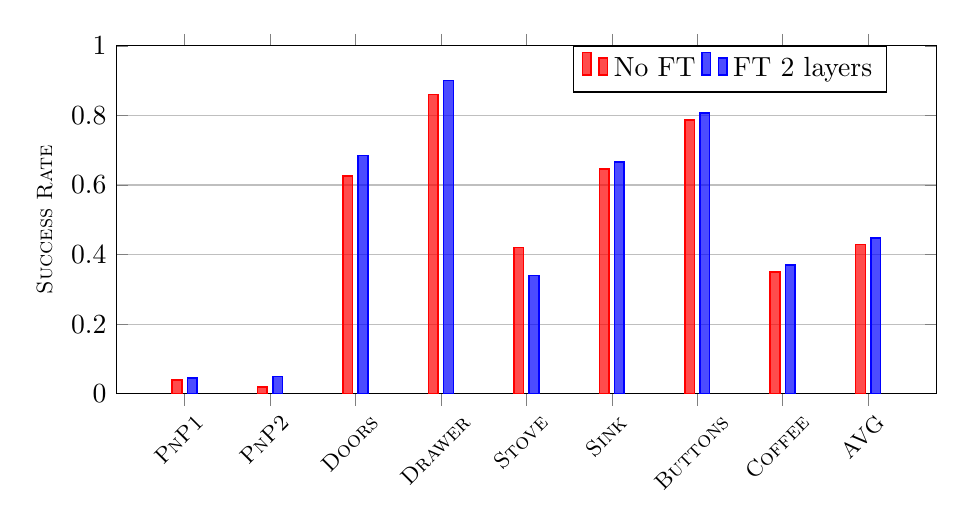
\begin{tikzpicture}[baseline]
        % \definecolor{red}{RGB}{214,39,40}
        % \definecolor{blue}{RGB}{31,119,180}
        
        \begin{axis}[
            ybar,
            height=6cm, width=12cm,
            bar width=3.5pt,
            ylabel=Success Rate,
            ylabel style={
                font=\footnotesize\scshape
            },
            ymin=0, ymax=1,
            legend style={at={(0.748, 1)}, anchor=north, legend columns=-1},
            symbolic x coords={PnP1, PnP2, Doors, Drawer, Stove, Sink, Buttons, Coffee, AVG},
            xtick=data,
            xticklabel style={
                rotate=45,
                font=\footnotesize\scshape,
                yshift=3pt,
            },
            ymajorgrids
        ]
        
        \addplot [
            draw=red,
            fill=red,
            line width=.2mm,
            fill opacity=0.7
        ] coordinates {
            (PnP1, 0.0400)
            (PnP2, 0.0200)
            (Doors, 0.6250)
            (Drawer, 0.8600)
            (Stove, 0.4200)
            (Sink, 0.6467)
            (Buttons, 0.7867)
            (Coffee, 0.3500)
            (AVG, 0.4292)
        };

        \addplot [
            draw=blue,
            fill=blue,
            line width=.2mm,
            fill opacity=0.7
        ] coordinates {
            (PnP1, 0.0450)
            (PnP2, 0.0500)
            (Doors, 0.6850)
            (Drawer, 0.9000)
            (Stove, 0.3400)
            (Sink, 0.6667)
            (Buttons, 0.8067)
            (Coffee, 0.3700)
            (AVG, 0.4483)
        };

        \legend{No FT, FT 2 layers}
        \end{axis}
        
        \end{tikzpicture}
    }
    \caption{Success rates using different finetuning strategies for the pretrained SUGAR encoder.}
    \vspace{-10pt} 
    \label{fig:ablation_sugar_ft}
\end{figure}


% \subsection{Ablation on pretrained clip features}